\section{Results}
\subsection{Top Providers}
Analyzing the number of occurrences of each domain name in the Adobe and Gawker 
email leaks gave us an idea of how many users use each provider.  The ordering 
and the exact numbers of the top domains differ somewhat, but there is some 
agreement between them.  For example, six of the top ten domains are the same 
for both sources (hotmail.com, gmail.com, yahoo.com, aol.com, comcast.net, and 
mail.ru).  For each of the top providers, we ran our scanner as outline 
above.  The results are summarized in the tables \ref{table:adobe} and 
\ref{table:gawker}.

The two most striking results from these tables are that the majority of users 
(\textgreater60\%) get service from just twenty email providers, and that at least half of 
the top email providers don’t provide any support for TLS when receiving emails.  
The biggest offender appears to be hotmail.com, which also hosts the MX servers 
for a number of other very large domains (e.g. hotmail.fr, outlook.com, msn.com, 
live.com).

\begin{table}
    \caption{Adobe Leak}
    \centering
    \label{table:adobe}
    \begin{tabular}{|l|l|l|l|}
        \hline
        Domain & \% Users & ESMTP & TLS \\
        \hline
        hotmail.com & \textgreater21.36 & Yes & No \\
        gmail.com & \textgreater15.76 & Yes & Yes \\
        yahoo.com & \textgreater11.69 & Yes & Yes \\
        aol.com & 2.28 & Yes & Yes \\
        comcast.net & 0.82 & Yes & No \\
        mail.ru & 0.82 & Yes & No \\
        web.de & 0.8 & Yes & Yes \\
        qq.com & 0.63 & Yes & No \\
        gmx.de & 0.63 & Yes & Yes \\
        naver.com & 0.43 & Yes & No \\
        \hline
    \end{tabular}
\end{table}

\begin{table}
    \caption{Gawker Leak}
    \centering
    \label{table:gawker}
    \begin{tabular}{|l|l|l|l|}
        \hline
        Domain & \% Users & ESMTP & TLS \\
        \hline
            gmail.com & \textgreater32.24 & Yes & Yes \\
            yahoo.com & \textgreater20.46 & Yes & Yes \\
            hotmail.com & \textgreater15.66 & Yes & No \\
            aol.com & 3.81 & Yes & Yes \\
            comcast.net & 1.5 & Yes & No \\
            mac.com & 1.08 & Yes & No \\
            verizon.net & 0.47 & Yes & No \\
            cox.net & 0.41 & Yes & No \\
            earthlink.net & 0.38 & Yes & No \\
            mail.ru & 0.3 & Yes & No \\
            naver.com & 0.43 & Yes & No \\
        \hline
    \end{tabular}
\end{table}

\subsection{TLS Support}
We first looked at just the proportion of email providers that support the 
STARTTLS command, ranked in order of number of users (as found in the Adobe 
leak).  We already know from figure \ref{server_tls} that of the top 10, only 50% 
support TLS.  As can be seen in figure \ref{sever_tls}, of the top 2000 providers, 
only 47.94\% support TLS.  We were surprised to see, however, that support for 
TLS actually increases as we looked at more and more providers, such that of the 
top 20,000 providers, 57.63\% supported TLS, and at 100,000 the number leveled 
off around 62.75\%.  We’re not entirely sure why we see this result, but one 
possible explanation is that many smaller, less-used email providers use Google 
mail servers, which support TLS, instead of setting up their own.

\begin{figure}
    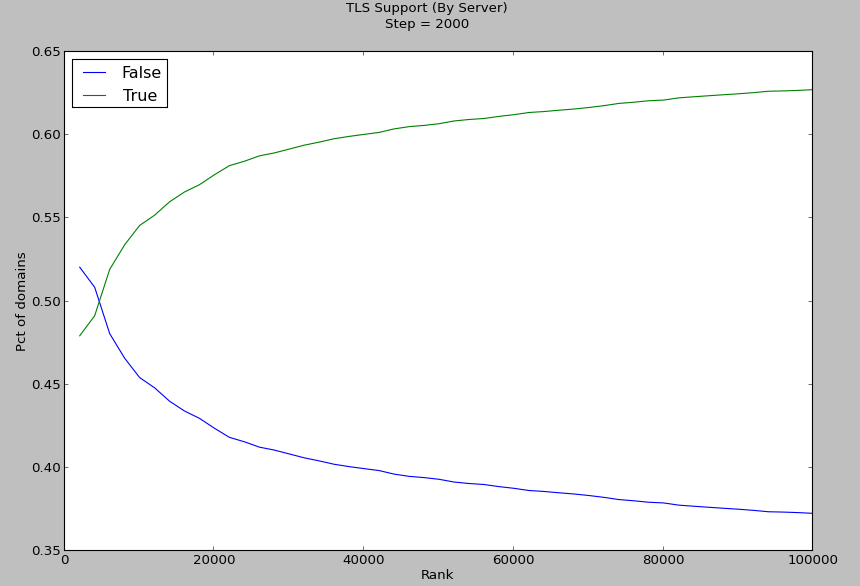
\includegraphics[width=3.0in]{images/server_tls.png}
    \caption{TLS Support by Server}
    \label{server_tls}
\end{figure}

\begin{figure}
    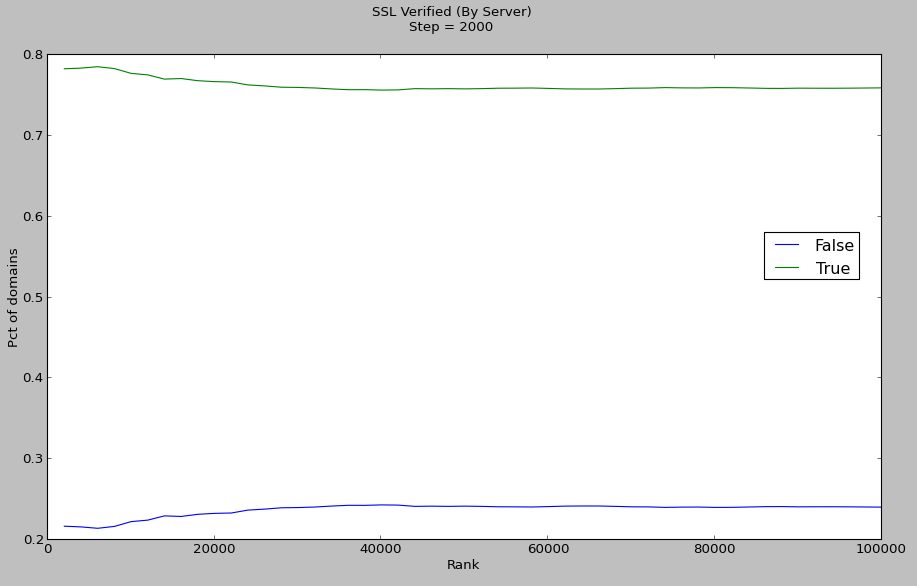
\includegraphics[width=3.0in]{images/server_verified.png}
    \caption{Valid SSL Cert by Server}
    \label{server_verified}
\end{figure}

\begin{figure}
    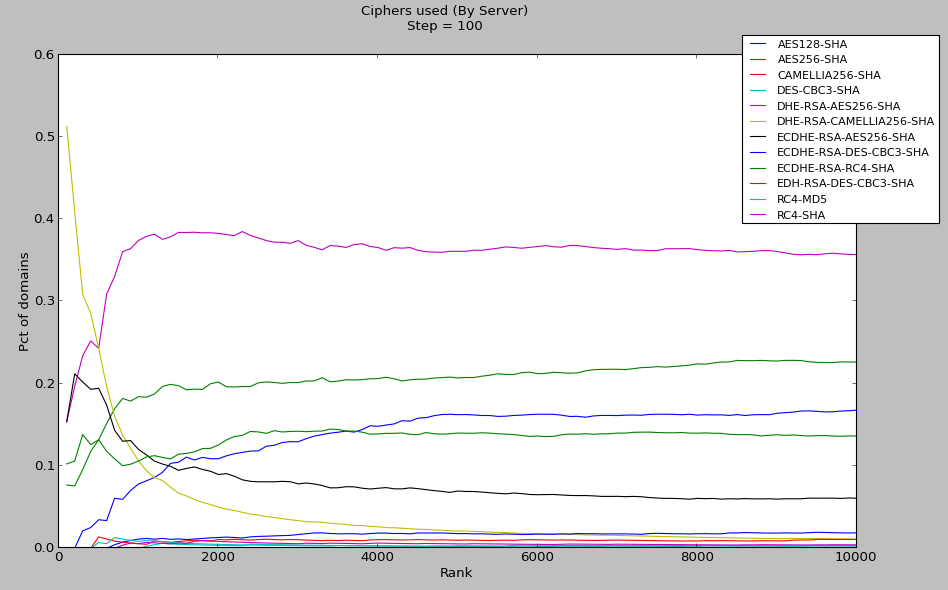
\includegraphics[width=3.0in]{images/server_ciphers.png}
    \caption{Cipher by Server}
    \label{server_ciphers}
\end{figure}

When we look at the proportion of actual users that have TLS support, however, 
the numbers are not quite as positive.  Looking at just the top 10 providers, 
only 52.72\% of users have a provider that supports TLS, and looking at our whole 
dataset that number goes down to 50.13\%.  That would suggest that of all the 
email users (at least, the ones who register with Adobe), only half receive 
emails with any encryption.  The numbers derived from the Gawker leak are 
considerably better (75.28\% for top 10, 71.84\% support for all providers) but 
again, we consider this source to be less representative of an international 
user base and more of an American (or at least Anglophone) user base.  In either 
case, this still implies that at most about 72\% of email users receive encrypted 
emails.

\subsection{Valid Encryption}
Based on the results of the previous section, we know that about 62\% of domains 
(covering between 50\% and 72\% of users) ostensibly support TLS, but we wanted to 
determine if those connections were really secure.  To do this, we opened secure 
connections to the SMTP servers and collected security certificates and cipher 
information.  Of the providers that support TLS, we found that only 75.9\% of 
them have valid certificates (i.e. they were signed by a trusted CA).  However, 
when looking at the proportion of users who use those providers, the numbers are 
much more positive: according to the Adobe leak, 98\% of users that use TLS have 
valid certificates, and according to the Gawker leak, 99.44\% use valid 
certificates.

We also examined the types of ciphers being used by providers who support TLS to 
see if many were using algorithms with known weaknesses. We found eleven ciphers 
used by the servers in our study; figure \ref{cipher_pie}. The only ciphers found that 
have known weaknesses are RC4-MD5 and RC4-SHA, together they are used by less 
than 0.06\% of the servers in this study.

\begin{figure}
    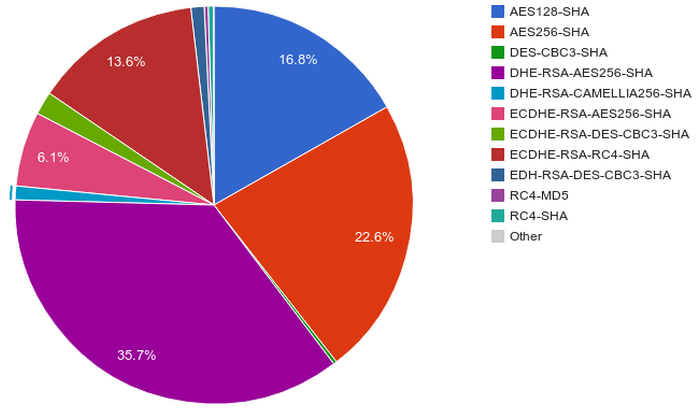
\includegraphics[width=3.0in]{images/pie_ciphers.png}
    \caption{Cipher Pie (Yum!)}
    \label{cipher_pie}
\end{figure}

\subsection{Overall Findings}
When looking at the ESMTP, TLS, and certificates use among all of the top 
million email providers Figure \ref{overall} we find that almost all 
providers support ESMTP with an adoption rate of 99.29\%. TLS support is only 
found on just over half of the providers at 54.58\%. Only 42.45\% of all 
providers, or 77.84\% of the providers with TLS, have a valid SSL 
certificate.

\begin{figure}
    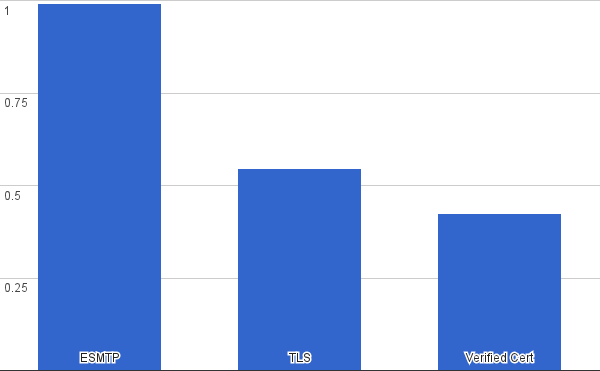
\includegraphics[width=3.0in]{images/bar_overall.png}
    \caption{Overall Picture}
    \label{overall}
\end{figure}

\subsection{Analysis of SMTP Headers}
After determining the state of security for one million email domains, we 
examined what effect that actually has when sending emails between domains by 
tracing the Received field of SMTP headers.  The results can be seen for seven 
of the top ten email providers in Figure \ref{email_analysis}, which shows the sender and 
receiver domains along with the protocol/encryption information for the 
inter-domain hop of the message.  Of those seven, all but hotmail.com and 
mail.ru support TLS.

\begin{figure*}
    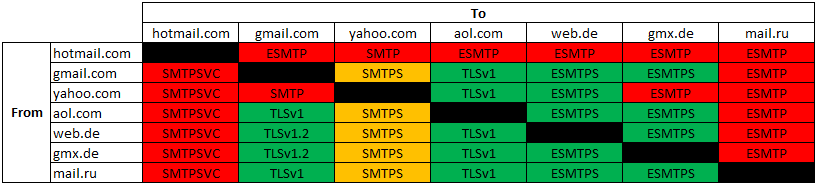
\includegraphics[width=6.0in]{images/email_analysis.png}
    \caption{SMTP Headers}
    \label{email_analysis}
\end{figure*}

The most obvious result is that the domains that do not support the STARTTLS 
command do not receive messages with encryption, which was to be expected.  A 
somewhat surprising result was that hotmail.com, which does not support TLS on 
incoming emails, also does not use TLS on its outgoing emails.  However, mail.ru 
uses the encryption settings of the destination server, even though it does not 
use encryption on incoming emails.  An even more surprising discovery was that 
yahoo.com did not use encryption when sending to gmail.com or gmx.de, even 
though all three domains support TLS.

We were somewhat unsure as to the level of encryption provided on emails bound 
for yahoo.com.  Headers with explicit cipher information were obviously sent 
with encryption, and IANA defines the ESMTPS parameter as indicating ESMTP 
with STARTTLS\cite{mail}. We assume that SMTPS similarly indicates that STARTTLS (or some other 
encryption mechanism) was used, but there is no official SMTPS parameter.

The implication of these results is that, while approximately 60\% of domains 
support TLS on incoming messages, not all MTAs actually make use of it when 
sending to those servers.  It is impossible to tell just what percent of 
email traffic is unencrypted without looking at the actual numbers of emails 
moving between different domains.  However, if only 50\% of users are on 
providers that support TLS on incoming messages and not all domains actually 
make use of that encryption when sending to those providers, it is 
reasonable to assume that at most 50\% of users are actively using 
encryption, and the number is probably somewhat lower.

\subsection{Outsourced Mail}
Many of the top domains actually share a common set of SMTP servers. This is due 
to providers such as Google and Microsoft who host email for domains owned by 
other companies. When we looked at who hosted the email of the top million 
providers we saw that the majority of email was being hosted by the five 
companies listed in table \ref{table:top_servers}. Here we see that Google hosts 
the most with 11\% of the domains email. The values listed in table 
\ref{table:top_servers} represent the lower bound of the amount of domains each 
provider is in control of.

\begin{table}
    \caption{Top Mail Servers by Domain}
    \centering
    \label{table:top_servers}
    \begin{tabular}{|l|l|}
        \hline
        Provider & \% of Domains \\
        \hline
        Google & 11.03\% \\
        Microsoft & 3.45\% \\ 
        Godaddy & 2.06\% \\
        MX Logic & 1.58\% \\
        RackSpace & 1.32\% \\
        \hline
    \end{tabular}
\end{table}

